\chapter{\label{III-C}Centraliser les référentiels de l’INA dans le \ldd: l'exemple de l'alignement de deux référentiels de personnes physiques}
\titreEntete{Aligner deux référentiels de personnes physiques}

%intro
\lettrine{L}a \ac{ddcol} possède un unique référentiel de personnes physiques, comme nous avons pu le constater plus tôt\footnote{Voir \reference{I-C-3} et \reference{II-C-3}.}. Le \ldd étant un \ac{led}, il tire son intérêt de la mise en commun de différentes bases de données et jeux de données. Ainsi, c'est l'ensemble des données et des métadonnées de l'\ac{ina} qui entrent dans ce \textit{Lac}: la base de données de la \ac{dj} fait alors l'objet de ce processus de migration vers le \ldd. Cependant, bien que la \ac{dj} représente un silo de données, distinct de celui de la \ac{ddcol}, ils partagent tout de même certaines caractéristiques comme l'utilisation massive de personnes physiques, qui sont réunies dans chaque service dans un référentiel.\\

La migration des données de la \ac{ddcol} s'achève à la fin de l'année 2020 et laisse la place à celle de la \ac{dj}: afin d'éviter toute redondance de concepts dans le \ldd, il convient de rechercher pour une personne physique de la \ac{dj} son équivalent dans le \ldd --- par conséquent dans l'ancien référentiel des personnes physiques et morales de la \ac{ddcol} qui a été déconstruit sous forme de concepts\footnote{Voir \reference{III-B}.}. L'exécution de cet alignement montre à lui seul les problématiques liées au langage naturel, ainsi que la nécessaire présence humaine qui doit superviser les résultats issus d'une automatisation de tâches.

\section{\label{III-C-1}Des jeux de données différents en de multiples points}
\titreEntete{Des jeux de données différents}

%intro
L'alignement des personnes physiques de la \ac{ddcol} avec Wikidata avait déjà démontré l'importance de la donnée structurée afin de créer des points de contacts entre les deux jeux de données et de procéder à leur alignement. Les problématiques liées à la graphie et aux différences de structure ont aussi compliqué cet alignement. Dans le cadre de la mise en relation entre le référentiel des personnes physiques de la \ac{dj} avec celui de la \ac{ddcol}, ces points de contact sont réduits au minimum et peuvent interroger quant à la possibilité de réaliser des alignements sûrs, ou les plus sûrs possibles.

\subsection{\label{III-C-1-a}Enjeux}
\titreEntete{Enjeux}

Le \ldd n'étant pas conçu à partir des\index[ref]{led@Linked Enterprise Data (LED)!ldd@Lac de données (INA)}\index[ref]{modelisation@Modélisation!ldd@Lac de données (INA)} besoins métier mais des données, le référentiel des personnes physiques de la \ac{dj}, se présentant sous la forme d'une table \textit{PERSONNE} de la base de données, ne peut pas être conservé dans sa structure actuelle. En effet, il est uniquement adapté aux besoins de la \ac{dj} et ne correspond pas aux usages que pourrait en faire la \ac{ddcol} ou l'utilisateur final des applications de l'\ac{ina}. Afin d'intégrer ce référentiel dans le \textit{Lac}, il est nécessaire de l'aligner avec les concepts existants, issus du référentiel des personnes physiques de la \ac{ddcol}. Ainsi, un double enrichissement a lieu, celui des concepts par les données de la \ac{dj}, et celui de la \ac{dj} par les données des concepts. Cependant, cet enrichissement devient invisible dans le \ldd puisqu'il n'y a plus de notion de référentiel, et que les distinctions entre \ac{dj} et \ac{ddcol} sont volontairement effacées au profit d'une structure de données plus souple.\\

Cet alignement a pour finalité l'ajout d'un lien \textit{provenance--\ac{dj}} à un concept quand le matricule de la \ac{dj} et le concept sont identiques, ou bien la détection des nombreuses personnes de la \ac{dj} qui ne sont pas des concepts. En effet, la \ac{dj} ayant pour fonction de repérer les ayants-droits et ouvrants-droits de personnes liées à un extrait audiovisuel, ceux-ci ne sont, par conséquent, pas spécifiquement dans la description des documents audiovisuels réalisée par la \ac{ddcol} car ils n'interviennent à aucun moment dans ces documents. Ainsi, nombreuses sont les personnes de la \ac{dj} qui n'ont pas d'équivalent dans la \ac{ddcol} et qu'il est nécessaire de repérer afin de leur créer \textit{in fine} un concept dans le \index[ref]{led@Linked Enterprise Data (LED)!ldd@Lac de données (INA)}\index[ref]{modelisation@Modélisation!ldd@Lac de données (INA)}\ldd.\\

Cette différence entre les jeux de données montre une nouvelle fois comment se sont formées les bases de données --- selon les usages et les besoins --- qui sont à migrer dans le \index[ref]{led@Linked Enterprise Data (LED)!ldd@Lac de données (INA)}\index[ref]{modelisation@Modélisation!ldd@Lac de données (INA)}\ldd: à cause de cette différence, il devient difficile d'estimer l'efficacité et le rendement du processus d'alignement qui va être réalisé. En effet, connaître la raison de l'absence d'alignement de certains matricules des personnes de la \ac{dj} sera uniquement possible par une action humaine. Face à ces enjeux et aux problématiques soulevées par le seul historique des bases de données, l'alignement des deux référentiels comporte plusieurs difficultés supplémentaires déjà évoquées dans les chapitres précédents.

\subsection{\label{III-C-1-b}Points de contact}
\titreEntete{Points de contact}

Trouver des points de contact entre deux jeux de données, plus encore entre deux référentiels, est essentiel lors d'un alignement: plus ces points de contact sont nombreux, plus les comparaisons sont nombreuses et les alignements sûrs. Cependant, les référentiels de la \ac{ddcol} et la \ac{dj} n'en partagent que peu --- sept. De plus, ces points de contact nécessitent la présence de l'information de chaque côté, ce qui est peu la cas entre la \ac{dj} et la \ac{ddcol}.\\

Dans le \index[ref]{led@Linked Enterprise Data (LED)!ldd@Lac de données (INA)}\index[ref]{modelisation@Modélisation!ldd@Lac de données (INA)}\ldd, les concepts disposent notamment d'attributs indiquant le nom, le sexe, les dates de naissance et de décès, ainsi que la note qualité. Cette note qualité n'étant pas scindée dans le \ldd, il est nécessaire, dans cet alignement, d'en extraire la fonction, ou les fonctions, de la personne, en supprimant la mention des pays d'exercice.\\

Si la \ac{dj} dispose de nombreuses données personnelles pour mener à bien ses missions, les données permettant un alignement documentaire sont plus restreintes: hormis le nom et le sexe, seule une date de décès est disponible, ainsi qu'une contribution. En effet, seule la date de décès intéresse le service juridique pour ses applications dans le droit et le reversement des droits aux ayants-droits ou ouvrants-droits: conserver une date de naissance n'a par conséquent aucun usage dans la \ac{dj}.

\noindent Le référentiel des personnes de la \ac{dj} présente une petite normalisation avec les contributions: celles-ci ne sont pas du texte libre, mais du texte contrôlé et choisi parmi une liste d'une vingtaine d'entrées. Ce contrôle du vocabulaire permet, dans l'alignement, des rendements meilleurs après, nous le verrons, un traitement préalable des données des notes qualité de la \ac{ddcol}.\\

Cependant, les points de contact identifiés pour la \ac{dj} et la \ac{ddcol} sont peu nombreux, ce qui complique la détection des homonymes et diminue la fiabilité des alignements futurs.

\subsection{\label{III-C-1-c}Divergences}
\titreEntete{Divergences}

En plus de ces difficultés sur la quantité des points de contact, les deux référentiels diffèrent par leurs structures et leurs graphies. Tout d'abord, les niveaux de description des mêmes attributs sont différents. En effet, alors que le nom du concept du \index[ref]{led@Linked Enterprise Data (LED)!ldd@Lac de données (INA)}\index[ref]{modelisation@Modélisation!ldd@Lac de données (INA)}\ldd est composé de la forme \og \textit{Nom, Prénom}\fg{}, l'état-civil stocké à la \ac{dj} est divisé en deux attributs: un nom et un prénom. Ainsi, avant d'effectuer l'alignement, il est nécessaire de scinder le nom du concept afin de récupérer le nom et le prénom séparément.

\noindent Le jeu de données de la \ac{dj} offre également deux autres attributs, les pseudos de nom et de prénom de chaque personne. Afin d'utiliser ces deux attributs supplémentaires, il est nécessaire de leur trouver un point de contact dans les concepts issus de la \ac{ddcol}: ainsi, il a été considéré qu'un nom de concept ne possédant pas de virgule est un pseudo. Par conséquent, ce pseudo, issu des concepts, peut être comparé avec le pseudo du nom de la \ac{dj}\footnote{Dans les données de la \ac{dj}, c'est le pseudo-nom qui comporte le pseudonyme courant d'une personne; l'attribut pseudo prénom n'est utilisé que pour indiquer une variante du prénom de cette personne.}.\\

En plus de ces différences de niveaux de description, les graphies ne sont pas les mêmes. D'abord, les données de la \ac{dj} sont en majuscules, alors que celles de la \ac{ddcol} sont en minuscules. Si cette difficulté n'est pas majeure, elle nécessite tout de même un traitement dans l'ETL avant de pouvoir procéder à un alignement. De même, afin d'éviter toute variation dans des chaînes de caractères renvoyant à une même personne mais aux graphies différentes, les accents et la ponctuation sont retirés. Les dates, commee lors des alignements décrits dans les chapitres précédents, sont réduites à la seule année.

\noindent La difficulté majeure, posée dans l'alignement de deux référentiels de personnes, est la graphie et l'utilisation des particules des noms. En effet, l'utilisation des particules n'est pas normalisée dans l'Institut, ce qui conduit à la présence de \nP{Louis de }{Funès} dans la \ac{ddcol}, alors que la \ac{dj} conserve la forme \nP{Louis}{de Funès}. Les pratiques d'écriture des noms à particules étant constantes à la \ac{ddcol}, il est possible de transférer cette particule\footnote{Cette particule n'est pas exclusivement \textit{de}, elle peut être de l'une des formes suivantes: \textit{de, des, du, de la}} dans le nom afin d'obtenir  \nP{Louis}{de Funès} dans chaque jeu de données.\\

Enfin, afin de donner aux alignements une plus grande fiabilité, il est essentiel de prendre en compte le texte des notes qualité pour le comparer avec les contributions de la \ac{dj}. Les notes qualité de la \ac{ddcol} comportant plus de vingt mille fonctions différentes, il n'est pas possible de les faire correspondre chacune avec l'une des contributions de la \ac{dj}. Pour cela, seules les contributions et les fonctions des notes qualité les plus courantes ont fait l'objet d'un alignement manuel pour faciliter l'alignement automatique qui va suivre; cinq de ces contributions ont ainsi été pu être traitées:
\begin{itemize}
	\item le terme \textit{Journalisme} de la \ac{dj} est remplacé par \og journaliste\fg{};
	\item \textit{Artiste interprètre} est remplacé par \og chanteu\fg{}\footnote{Les terminaisons sont enlevées dans ces termes de remplacement afin de prendre en compte les variantes de graphie liées au pluriel et au féminin que l'on peut trouver dans les fonctions de la \ac{ddcol}.}
	\item \og realisat\fg remplace \textit{Réalisation}
	\item \og composit\fg remplace \textit{Composition musicale}
	\item enfin, \textit{Réalisation associée} est remplacé par \og realisat\fg{}
\end{itemize}
\medskip
Les chanteurs, les compositeurs, les réalisateurs et les journalistes étant les fonctions les plus courantes dans les deux jeux de données, elles ont été repérées puis traitées. Cependant, une majorité de fonctions ne pourra pas être alignée avec les contributions de la \ac{dj}, et par conséquent limitera la confiance accordée aux alignements.


%conlu
\bigskip
\bigskip
La centralisation de référentiels et de données est nécessaire pour les systèmes documentaires, mais la reprise de ces référentiels et de ces données peut être compliquée par les structures et les normes divergentes selon les jeux de données. Cette absence d'uniformisation annonce déjà des résultats faibles et limités dans la confiance qui peut être accordée. Dans le cas de l'alignement des référentiels de personnes physiques de la \ac{dj} et de la \ac{ddcol} à l'\ac{ina}, les points de contacts sont peu nombreux et peu spécifiques\footnote{Voir \reference{table_contact_dj_ddcol}.}.

\begin{table}[!h]
	\centering
	\begin{tabular}{|c|c|}
		\hline
		\textbf{\ac{dj}} & \textbf{\ac{ddcol}}\\ \hline
		Nom&Nom\\ \hline
		Prénom&Prénom\\ \hline
		Pseudo nom&Pseudo\\ \hline
		Pseudo prénom&\\ \hline
		Sexe&Sexe\\ \hline
		Date de naissance&Date de naissance\\ \hline
		Contribution&Fonction\\ \hline
	\end{tabular}
	\caption[Points de contact entre les référentiels de la \ac{dj} et de la \ac{ddcol}]{Points de contact entre les référentiels de la \ac{dj} et de la \ac{ddcol}}
	\label{table_contact_dj_ddcol}
\end{table}

\section{\label{III-C-2}Établir une méthodologie particulière d'alignement}
\titreEntete{Une méthodologie particulière}

%intro
En raison des difficultés identifiées dans la \reference{III-C-1}, un alignement simple, n'apportant aucune indication de fiabilité, n'est pas possible. De même, les alignements réalisés dans les chapitres précédents utilisent chacun les jeux de données initiaux jusqu'à la fin du traitement, sans en retirer au fur et à mesure les concepts qui viennent d'être alignés. L'alignement des référentiels de la \ac{ddcol} et de la \ac{dj} se distingue des précédents par la nécessité d'une méthodologie particulière, basée sur un indice de confiance attribué à chaque alignement, et sur une succession d'étapes, représentant les niveaux de confiance apportés au type de jointure utilisé.

\subsection{\label{III-C-2-a}Créer un indice de confiance pour chaque alignement}
\titreEntete{Créer un indice de confiance}

Les points de contact entre les jeux de données n'ont pas tous la même valeur dans un alignement. En effet, l'état civil d'une personne, bien qu'essentiel dans un alignement, peut conduire à aligner deux homonymes: c'est pourquoi les points de contact comme les noms, les prénoms ou les pseudos peuvent être considérés comme ayant une faible valeur dans le processus d'alignement. De plus, leur octroyer une valeur forte conduirait à surévaluer les alignements réalisés sur la simple comparaison des noms et prénoms sans autre point de comparaison par rapport aux alignements qui n'auront pas été possibles.\\

En revanche, la valeur des points de comparaison significatifs est considérée comme forte: il s'agit de la date de décès ou de la contribution. En effet, la probabilité que les états civils et les dates de décès de deux homonymes soient identiques est très faible, ce qui peut permettre de donner à cet alignement une valeur plus forte. De même, la correspondance entre une contribution et une fonction est considérée comme très fiable quand les états civils ont déjà été rapprochés: pour cette raison, le point de comparaison sur la contribution est celui qui possède l'indice de confiance le plus élevé, puisqu'il est le point le plus spécifique, et le plus difficile à faire correspondre.\\

Enfin, la comparaison du sexe permet également d'augmenter la fiabilité d'un alignement. Dans la majorité des alignements qui sont réalisés, la comparaison peut sembler évidente à l'humain, mais dans certains cas, comme pour les prénoms \textit{Dominique}, elle est nécessaire et permet la conservation ou non de l'alignement.\\

L'indice de confiance permet une priorisation des points de comparaison, une hiérarchisation de ces derniers. Il se forme à partir de la somme des scores de chaque point de comparaison. Ainsi, dans le cas de l'alignement des référentiels de personnes de la \ac{dj} et de la \ac{ddcol}, l'indice de confiance varie entre 0 --- quand l'alignement n'a pas pu être réalisé --- et 9 --- quand tous les points de comparaison ont été réalisés avec succès --- selon les scores de la \reference{table_scores}.
\begin{table}[!h]
	\centering
	\begin{tabular}{|c|c|}
		\hline
		\textbf{Point de comparaison}&\textbf{Score}\\ \hline
		Nom&1\\ \hline
		Prénom&1\\ \hline
		Pseudo nom&1\\ \hline
		Pseudo prénom&1\\ \hline
		Sexe&1\\ \hline
		Date de décès&2\\ \hline
		Contribution&2\\ \hline
	\end{tabular}
	\caption{Scores attribués à chaque point de comparaison}
	\label{table_scores}
\end{table}

\subsection{\label{III-C-2-b}Des étapes exclusives}
\titreEntete{Des étapes exclusives}

L'attribution d'un indice de confiance ne permet de résoudre que la problématique de l'évaluation finale des alignements. Il subsiste néanmoins une seconde problématique, celle de la présence dans les alignements réalisés de doublons, c'est à dire de personnes de la \ac{dj} alignés avec plusieurs concepts. Une solution pourrait être de supprimer les alignements présents dans ce cas. Or, ce cas survient fréquemment: supprimer les alignements concernés réduirait la quantité de résultats finaux.\\

Ainsi, après une première priorisation des points de comparaison, il est nécessaire d'effectuer ensuite une priorisation des combinaisons de ces points de comparaison. Quatre étapes principales ont été identifiées et constituent cette priorisation.

\noindent D'abord, les alignements réalisés avec le nom, le prénom, les pseudos et la correspondance des fonctions sont considérés comme ceux étant les plus sûrs pour effectuer les rapprochements entre les concepts de la \ac{ddcol} et les matricules de la \ac{dj}. Ces alignements, comme ceux des étapes suivantes, sont des jointures\footnote{Afin de ne récupérer que les alignements qui ont été réalisés, ces jointures sont de type \textit{inner join}.} entre les deux jeux de données réalisées dans l'ETL Talend avec le composant associé, un tMap (\reference{tmap_jointures}).
\begin{figure}[!h]
	\centering
	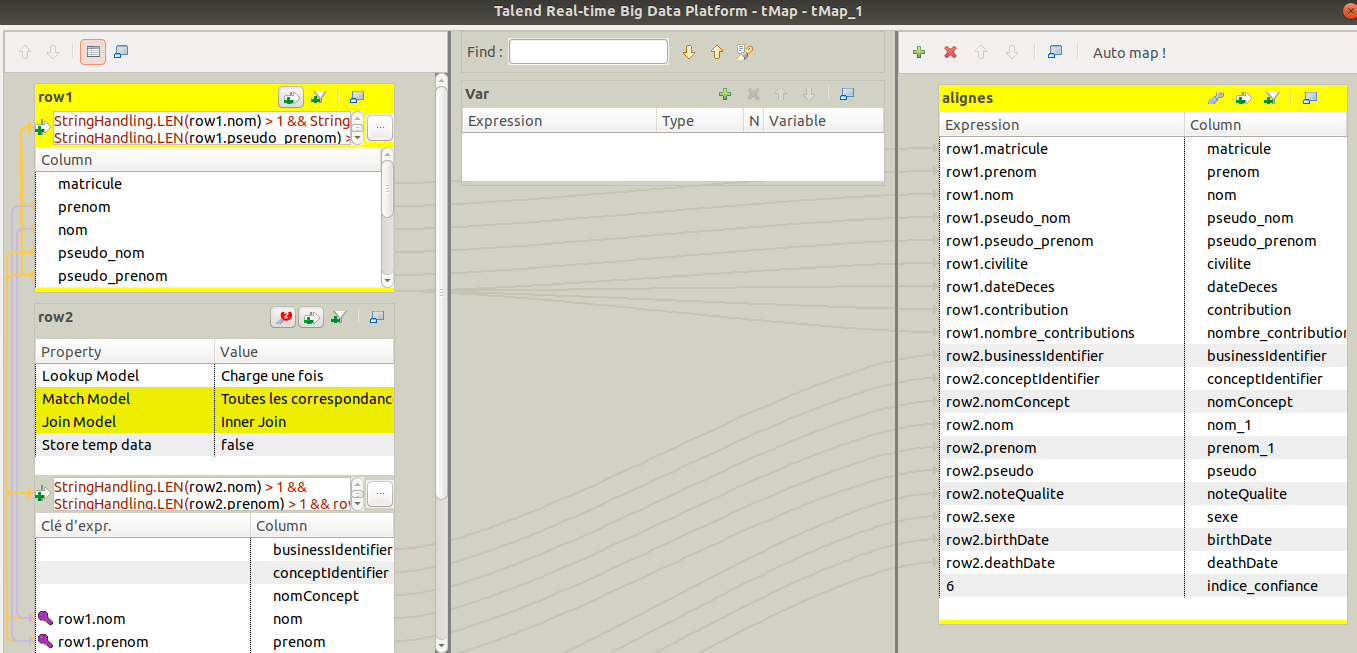
\includegraphics[width=16cm]{images/tmpa_jointure1_dj.png}
	\caption{L'alignement des personnes de la \ac{dj} et de la \ac{ddcol} pour une jointure dans un tMap de Talend.}
	\label{tmap_jointures}
\end{figure}

\noindent Ensuite, les alignements effectués avec le nom, le prénom et les pseudos, sans avoir pu faire correspondre les fonctions, sont la seconde étape.

\noindent La troisième étape, comme la quatrième, tente de rapprocher deux personnes en prenant en compte les différences de graphie qui peuvent exister. Ainsi, les alignements sont réalisés sur les pseudos, et sur le prénom de la \ac{dj} commençant par le prénom de la \ac{ddcol}\footnote{Une exception a été créé dans cette étape pour les prénoms \textit{Jean} et \textit{Anne}.}. Cette étape permet l'alignement d'une même personne ayant à la \ac{ddcol} le prénom \textit{Louis} et à la \ac{dj} le prénom \textit{Louis Marie}.

\noindent Enfin, l'ensemble des combinaisons possibles étant couvert, il est nécessaire d'effectuer une dernière étape pour effectuer non pas des alignements fiables --- ce qui est le but des trois premières étapes --- mais des alignements permettant d'apporter une aide à un opérateur humain en proposant plusieurs concepts qu'il est possible d'aligner avec un matricule. Ce rapprochement particulier, réalisé sur les seuls nom et prénom, autorise par conséquent la présence de plusieurs concepts alignés avec un même matricule, notamment dans le cas d'homonymes.\\

Distinguer ces quatre étapes permet, à l'issue de chacune d'elles, de récupérer ce qui n'a pas été aligné, tant du côté de la \ac{dj} et de la \ac{ddcol}, afin d'effectuer l'étape suivante avec uniquement ces données non alignées (\reference{orchestration}). Cette récupération évite de créer des alignements doubles avec des concepts différents entre les étapes. C'est également à l'issue de cette récupération que les résultats des jointures précédentes sont comparés afin de supprimer les matricules alignés plusieurs fois, et d'attribuer les scores pour le sexe et la date.\\
\begin{figure}[!h]
	\centering
	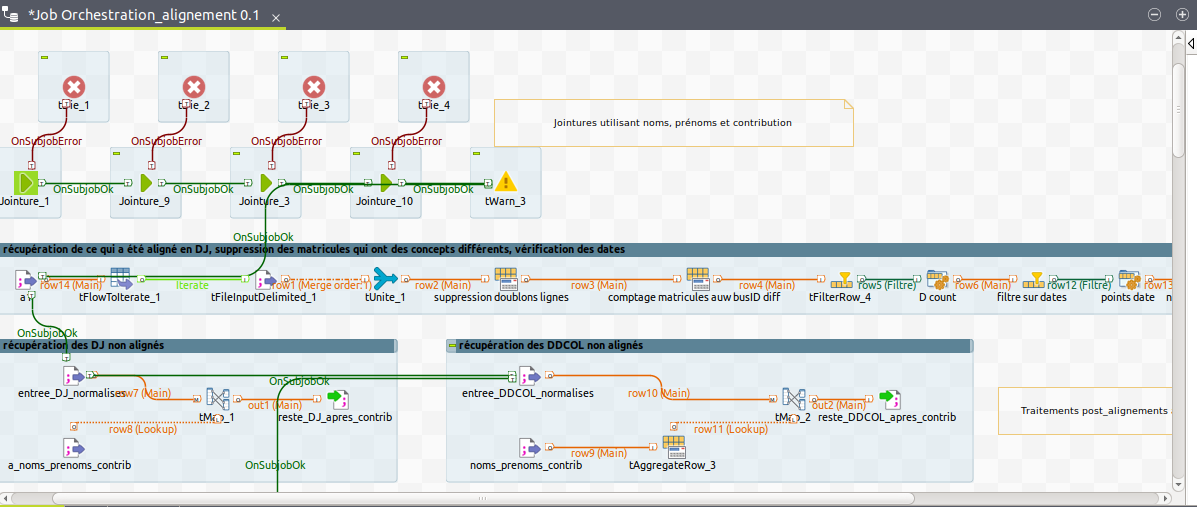
\includegraphics[width=16cm]{images/orchestration_partie1_dj.png}
	\caption{L'orchestration de la première étape dans l'ETL Talend.}
	\label{orchestration}
\end{figure}

Cependant, la limite de la récupération des matricules des personnes non alignées de la \ac{dj} et de la \ac{ddcol} est dans la priorisation qui a été faite des étapes. En effet, elle se base uniquement sur des critères définis en amont par un humain selon l'observation des cas généraux d'alignements: bien que ce soit une méthode apportant de la fiabilité aux alignements, cette fiabilité n'est pas nécessairement celle qui est la plus optimale. De même, cette récupération pourrait avoir lieu après chaque alignement de matricule: cela ajouterait néanmoins une nouvelle priorisation, basée sur l'ordre de passage, qui est plus arbitraire encore, puisque cet ordre de passage des matricules de la \ac{dj} dans le processus d'alignement n'est régi par aucun ordre significatif\footnote{Une base de données relationnelle n'étant pas ordonnée.}.

%conlu
\bigskip
\bigskip
Face aux nombreuses difficultés, l'indice de confiance et la priorisation des étapes permettent de réduire les mauvais alignements, et d'apporter une précision sur la fiabilité d'un alignement. Cependant, l'automatisation de ce processus présente des limites comme la définition de règles dirigeant le processus d'alignement. L'alignement des soixante-dix mille matricules de la \ac{dj} et des plus de trois cent mille concepts de la \ac{ddcol} ne peut pas être réalisé sur la base de quelques règles puis être considéré comme fiable.
\section{\label{III-C-3}Des résultats à la hauteur des données initiales}
\titreEntete{Des résultats à la hauteur des données initiales}

%intro
Les résultats de l'automatisation d'un processus de traitement de données dépend entièrement de la qualité des données initiales. Les difficultés propres aux différences de structures entre les jeux de données ou aux différences de graphie, additionnées à celles posées par la volonté d'avoir des alignements fiables et sans doublons, sont autant de facteurs qui réduisent l'efficacité de l'alignement automatique de deux référentiels.\\

Dans le cas de l'alignement des référentiels de personnes de la \ac{dj} et de la \ac{ddcol}, les résultats reflètent les difficultés rencontrées, tant dans les quantités de résultats que dans les indices de confiance attribués. Cette hétérogénéité des résultats conduit à la nécessité d'une supervision humaine des alignements réalisés et non réalisés.

\subsection{\label{III-C-3-a}Des résultats hétérogènes reflétant les multiples difficultés}
\titreEntete{Des résultats hétérogènes}

Environ soixante pour cent des matricules de personnes de la \ac{dj} ont trouvé leur équivalent dans la \ac{ddcol}. Ce résultat, bien que faible, reflète les difficultés rencontrées, ainsi que la spécificité des usages de chaque référentiel. En effet, la \ac{dj} utilise les personnes pour leur verser des droits, ce qui signifie alors que ces personnes ne sont pas spécialement des acteurs des documents conservés à la \ac{ddcol} pour lesquels le référentiel des personnes physiques a été créé. Il est par conséquent normal de ne pas pouvoir aligner tous les matricules de la \ac{dj} avec la \ac{ddcol}, cette dernière n'ayant pas besoin de conserver les ayants-droits de chaque personne du référentiel.

\begin{figure}[!h]
	\centering
	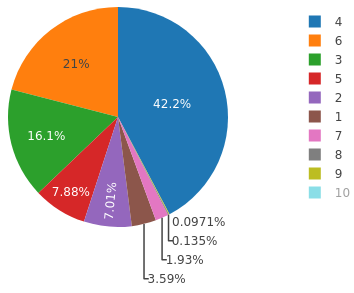
\includegraphics[width=8cm]{images/indices.png}
	\caption{Répartition des indices de confiance après les alignements entre les rééfrentiels de personnes de la \ac{dj} et de la \ac{ddcol}}
	\label{indices}
\end{figure}

La répartition des indices de confiance (\reference{indices}) reflète quant à elle à la fois la qualité des données initiales, ainsi que le processus d'alignement en lui-même. En effet, les différences de niveaux de précision dans les jeux de données initiaux conduisent à l'impossibilité d'utiliser certains points de comparaison, ce qui réduit l'indice de confiance: ces différences peuvent être une absence de données d'un côté de l'alignement, ou bien une divergence de graphie ou de structure qui n'a pas pu être corrigée lors du traitement préalable des données. Ainsi, l'indice \textit{4} est celui le plus présent en raison du faible nombre de points de comparaison qui le permettent: le nom, le prénom ainsi que la date ou une fonction suffisent à attribuer cet indice.\\

De plus, l'enchaînement des étapes entraîne également une diminution des indices de confiance: les étapes considérées comme prioritaires sont aussi celles qui utilisent les points de comparaison à la plus forte valeur. Ainsi, les indices de confiance attribués dans les alignements sont globalement inférieurs à cinq, et peu peuvent être considérés comme fiables quand l'indice est supérieur à cinq ou six.

\subsection{\label{III-C-3-b}Une supervision humaine nécessaire}
\titreEntete{Une supervision humaine nécessaire}

L'incertitude entourant la majorité des alignements conduit, comme cela est le cas pour le catalogage après la génération automatique de données, à utiliser une supervision humain. En effet, seule l'expertise et la réflexion d'un agent humain peut, ou non, confirmer les alignements produits. Seulement, cet agent humain va se heurter également à certaines problématiques posées dans l'automatisation: l'absence d'informations dans un matricule de la \ac{dj} ou dans un concept du \ldd ne permettra pas d'affirmer si les deux personnes alignées automatiquement sont réellement identiques et peuvent être associées.\\

Outre ce rejet ou cette acceptation des alignements réalisés automatiquement, la supervision humaine doit pouvoir modifier ce qui lui est proposé, ou bien pouvoir créer de nouveaux alignements. En effet, les jointures effectuées dans Talend\footnote{Elles sont au nombre de onze.} ne prennent pas en compte toutes les possibilités des deux jeux de données\footnote{Il existe quarante-deux (sept attributs sont disponibles dans la \ac{dj}, et six dans la \ac{ddcol}) jointures de stricte égalité possibles.} pour des raisons de fiabilité de ces possibilités dans le processus d'alignement. L'agent humain est seul capable de rechercher dans les données de la \ac{ddcol} un concept selon des critères que l'intelligence humaine offre: ils peuvent être l'inversion de deux lettres suite à une coquille dans la graphie, la francisation ou la traduction d'un terme étranger, l'inversion de deux prénoms, la connaissance d'un autre pseudonyme de la personne qui n'est pas spécifié dans les données de la \ac{dj}, \dots

%conlu
\bigskip
\bigskip
L'action humaine est toujours nécessaire, même avec un processus automatique d'alignement entre des données. Cette action est essentielle pour obtenir des données cohérentes et fiables dans un nouveau modèle de données. En effet, ces données étaient initialement cohérentes et sûres dans leurs bases de données respectives: elles doivent retrouver cette cohérence et cette fiabilité, même après un traitement automatique. Pour cela, la supervision humaine est nécessaire pour s'en assurer et proposer le cas échéant des solutions. 

%conclu
\bigskip
\bigskip
Dans le projet de centralisation des données de l'\ac{ina}, la centralisation des référentiels est indispensable, ces derniers étant devenus les pivots du système d'information. La conservation d'un référentiel utilisé par un seul jeu de données, celui de la \ac{dj}, ne correspond pas aux principes du \ac{led} et du \ldd. Ainsi, sa migration dans ce \textit{Lac} a nécessité un traitement important pour aboutir à l'alignement de ses matricules avec les concepts du \ldd. Face aux résultats de cet alignement, l'indice de confiance attribué offre une meilleure visibilité du travail effectué automatiquement, et permet aux superviseurs, qui sont nécessaires, d'approuver ou de refuser chaque alignement, afin d'éviter l'introduction d'erreurs dans le \ldd.